\subsection{Six-method mathematics comparison and held-out evaluation}\label{app:math-six}\label{app:language}
We extend the same Qwen2.5-7B/Llama-3.1-8B mathematics setup with four methods that vary adaptation structure. DoRA separates weight-vector magnitudes and directions, learning magnitudes alongside a low-rank directional update \citep{liu2024dora}. PiSSA and MiLoRA initialize the trainable factors from leading and trailing singular components, respectively \citep{meng2024pissa,wang2025milora}. In both cases, subtracting the initial low-rank component from the frozen base preserves the starting model. HRA learns a product of Householder reflections \citep{yuan2024hra}. In an input-side convention,
\begin{equation*}
 \bm W=\bm W_0\prod_{j=1}^{r_H}\bm H_j,
 \qquad \bm H_j=\bm I-2\frac{\bm v_j\bm v_j^{\!\top}}{\bm v_j^{\!\top}\bm v_j}.
\end{equation*}
The implementation uses the compact WY representation \citep{schreiber1989wy,likhosherstov2021cwy}, paired identity initialization and no Gram--Schmidt orthogonalization. Here $r_H$ counts Householder vectors. DoRA/PiSSA/MiLoRA use training ranks 7/14/28 for Qwen and 7/15/30 for Llama, with $\alpha=2r$. HRA uses 16/32/64 vectors. The capacity tiers approximately match trainable parameter counts. PiSSA/MiLoRA serialization expresses their final differences against the original base at rank $2r$. The tables report the actual training rank and trainable parameter count.

All methods use the same seven attention/MLP projection types, AdamW, batch 32, sequence length 768, 625 updates, cosine decay, warmup fraction 0.03, zero weight decay and gradient clipping at one. The original grid uses LRs $\{1,3,10,30,100\}\times10^{-5}$ and seeds 13/37/73. It contains 540 training outcomes, comprising 180 LoRA/OFT and 360 added-method runs. Qwen PiSSA r7 at LR $10^{-3}$, seed 73, diverged at step 55, leaving 539 final development evaluations. The group with two successful seeds is excluded from LR selection and complete-configuration frontiers.

\paragraph{Selection and test separation.}
One LR per model/method/capacity maximizes the exact total correct count across seeds on the fixed 1,000-problem, group-held-out GSM8K development panel. Ties choose the smaller LR. The resulting 36 configurations and 108 checkpoints are fixed before test evaluation, with one LR shared across seeds. Each checkpoint is evaluated on all 1,319 official GSM8K test problems. Prior test-set use for evaluation-harness development was separate from this selection. Generation uses the same native BF16 merged-adapter path, prompt and answer parser, greedy decoding, a 300-new-token cap, an 800-total-token cap and a 1,024-token engine context. The six-method intervention figures use development scores.

Retention reuses each run's recorded standard step-625 FineWiki-200 measurement, at length 768 and batch two. We report $\Delta\mathrm{NLL}=\mathrm{NLL}_{625}-\mathrm{NLL}_0$, using the corresponding pretrained reference. Smaller values indicate better general-text retention. We report sample SD across training seeds.

\begin{table}[!htbp]
\caption{Qwen2.5-7B results for all development-selected configurations from the original five-LR grid. Parameters are in millions. Ranks are training ranks (HRA counts Householder vectors). Accuracy is in percent, and $\Delta$NLL is the recorded FineWiki-200 NLL minus its matching pretrained value. LRs were selected using development accuracy only.}
\label{tab:math-selected-qwen}
\begin{center}
\setlength{\tabcolsep}{3pt}\renewcommand{\arraystretch}{1.12}
\begin{tabular*}{\linewidth}{@{\extracolsep{\fill}}lrcccc@{}}\toprule
Adapter & Params (M) & LR & Dev $\uparrow$ & Test $\uparrow$ & $\Delta$NLL $\downarrow$ \\ \midrule
\textcolor{LoRAColor}{LoRA} r7 & \result{math_grid_qwen_lora_7_0p001_params} & $1\times10^{-3}$ & $\result{math_grid_qwen_lora_7_0p001_dev_mean}_{\pm\result{math_grid_qwen_lora_7_0p001_dev_sd}}$ & $\result{math_grid_qwen_lora_7_0p001_test_mean}_{\pm\result{math_grid_qwen_lora_7_0p001_test_sd}}$ & $\result{math_grid_qwen_lora_7_0p001_forgetting_mean}_{\pm\result{math_grid_qwen_lora_7_0p001_forgetting_sd}}$ \\
\textcolor{LoRAColor}{LoRA} r14 & \result{math_grid_qwen_lora_14_1em05_params} & $1\times10^{-5}$ & $\result{math_grid_qwen_lora_14_1em05_dev_mean}_{\pm\result{math_grid_qwen_lora_14_1em05_dev_sd}}$ & $\result{math_grid_qwen_lora_14_1em05_test_mean}_{\pm\result{math_grid_qwen_lora_14_1em05_test_sd}}$ & $\result{math_grid_qwen_lora_14_1em05_forgetting_mean}_{\pm\result{math_grid_qwen_lora_14_1em05_forgetting_sd}}$ \\
\textcolor{LoRAColor}{LoRA} r28 & \result{math_grid_qwen_lora_28_3em05_params} & $3\times10^{-5}$ & $\result{math_grid_qwen_lora_28_3em05_dev_mean}_{\pm\result{math_grid_qwen_lora_28_3em05_dev_sd}}$ & $\result{math_grid_qwen_lora_28_3em05_test_mean}_{\pm\result{math_grid_qwen_lora_28_3em05_test_sd}}$ & $\result{math_grid_qwen_lora_28_3em05_forgetting_mean}_{\pm\result{math_grid_qwen_lora_28_3em05_forgetting_sd}}$ \\
\addlinespace[2pt]
\addlinespace[2pt]
\textcolor{OFTColor}{OFT} b32 & \result{math_grid_qwen_oft_32_0p0003_params} & $3\times10^{-4}$ & $\result{math_grid_qwen_oft_32_0p0003_dev_mean}_{\pm\result{math_grid_qwen_oft_32_0p0003_dev_sd}}$ & $\result{math_grid_qwen_oft_32_0p0003_test_mean}_{\pm\result{math_grid_qwen_oft_32_0p0003_test_sd}}$ & $\result{math_grid_qwen_oft_32_0p0003_forgetting_mean}_{\pm\result{math_grid_qwen_oft_32_0p0003_forgetting_sd}}$ \\
\textcolor{OFTColor}{OFT} b64 & \result{math_grid_qwen_oft_64_0p0003_params} & $3\times10^{-4}$ & $\result{math_grid_qwen_oft_64_0p0003_dev_mean}_{\pm\result{math_grid_qwen_oft_64_0p0003_dev_sd}}$ & $\result{math_grid_qwen_oft_64_0p0003_test_mean}_{\pm\result{math_grid_qwen_oft_64_0p0003_test_sd}}$ & $\result{math_grid_qwen_oft_64_0p0003_forgetting_mean}_{\pm\result{math_grid_qwen_oft_64_0p0003_forgetting_sd}}$ \\
\textcolor{OFTColor}{OFT} b128 & \result{math_grid_qwen_oft_128_0p0001_params} & $1\times10^{-4}$ & $\result{math_grid_qwen_oft_128_0p0001_dev_mean}_{\pm\result{math_grid_qwen_oft_128_0p0001_dev_sd}}$ & $\result{math_grid_qwen_oft_128_0p0001_test_mean}_{\pm\result{math_grid_qwen_oft_128_0p0001_test_sd}}$ & $\result{math_grid_qwen_oft_128_0p0001_forgetting_mean}_{\pm\result{math_grid_qwen_oft_128_0p0001_forgetting_sd}}$ \\
\addlinespace[2pt]
\addlinespace[2pt]
\textcolor{DoRAColor}{DoRA} r7 & \result{math_grid_qwen_dora_7_0p0003_params} & $3\times10^{-4}$ & $\result{math_grid_qwen_dora_7_0p0003_dev_mean}_{\pm\result{math_grid_qwen_dora_7_0p0003_dev_sd}}$ & $\result{math_grid_qwen_dora_7_0p0003_test_mean}_{\pm\result{math_grid_qwen_dora_7_0p0003_test_sd}}$ & $\result{math_grid_qwen_dora_7_0p0003_forgetting_mean}_{\pm\result{math_grid_qwen_dora_7_0p0003_forgetting_sd}}$ \\
\textcolor{DoRAColor}{DoRA} r14 & \result{math_grid_qwen_dora_14_0p0003_params} & $3\times10^{-4}$ & $\result{math_grid_qwen_dora_14_0p0003_dev_mean}_{\pm\result{math_grid_qwen_dora_14_0p0003_dev_sd}}$ & $\result{math_grid_qwen_dora_14_0p0003_test_mean}_{\pm\result{math_grid_qwen_dora_14_0p0003_test_sd}}$ & $\result{math_grid_qwen_dora_14_0p0003_forgetting_mean}_{\pm\result{math_grid_qwen_dora_14_0p0003_forgetting_sd}}$ \\
\textcolor{DoRAColor}{DoRA} r28 & \result{math_grid_qwen_dora_28_0p0001_params} & $1\times10^{-4}$ & $\result{math_grid_qwen_dora_28_0p0001_dev_mean}_{\pm\result{math_grid_qwen_dora_28_0p0001_dev_sd}}$ & $\result{math_grid_qwen_dora_28_0p0001_test_mean}_{\pm\result{math_grid_qwen_dora_28_0p0001_test_sd}}$ & $\result{math_grid_qwen_dora_28_0p0001_forgetting_mean}_{\pm\result{math_grid_qwen_dora_28_0p0001_forgetting_sd}}$ \\
\addlinespace[2pt]
\addlinespace[2pt]
\textcolor{PiSSAColor}{PiSSA} r7 & \result{math_grid_qwen_pissa_7_3em05_params} & $3\times10^{-5}$ & $\result{math_grid_qwen_pissa_7_3em05_dev_mean}_{\pm\result{math_grid_qwen_pissa_7_3em05_dev_sd}}$ & $\result{math_grid_qwen_pissa_7_3em05_test_mean}_{\pm\result{math_grid_qwen_pissa_7_3em05_test_sd}}$ & $\result{math_grid_qwen_pissa_7_3em05_forgetting_mean}_{\pm\result{math_grid_qwen_pissa_7_3em05_forgetting_sd}}$ \\
\textcolor{PiSSAColor}{PiSSA} r14 & \result{math_grid_qwen_pissa_14_3em05_params} & $3\times10^{-5}$ & $\result{math_grid_qwen_pissa_14_3em05_dev_mean}_{\pm\result{math_grid_qwen_pissa_14_3em05_dev_sd}}$ & $\result{math_grid_qwen_pissa_14_3em05_test_mean}_{\pm\result{math_grid_qwen_pissa_14_3em05_test_sd}}$ & $\result{math_grid_qwen_pissa_14_3em05_forgetting_mean}_{\pm\result{math_grid_qwen_pissa_14_3em05_forgetting_sd}}$ \\
\textcolor{PiSSAColor}{PiSSA} r28 & \result{math_grid_qwen_pissa_28_3em05_params} & $3\times10^{-5}$ & $\result{math_grid_qwen_pissa_28_3em05_dev_mean}_{\pm\result{math_grid_qwen_pissa_28_3em05_dev_sd}}$ & $\result{math_grid_qwen_pissa_28_3em05_test_mean}_{\pm\result{math_grid_qwen_pissa_28_3em05_test_sd}}$ & $\result{math_grid_qwen_pissa_28_3em05_forgetting_mean}_{\pm\result{math_grid_qwen_pissa_28_3em05_forgetting_sd}}$ \\
\addlinespace[2pt]
\addlinespace[2pt]
\textcolor{MiLoRAColor}{MiLoRA} r7 & \result{math_grid_qwen_milora_7_1em05_params} & $1\times10^{-5}$ & $\result{math_grid_qwen_milora_7_1em05_dev_mean}_{\pm\result{math_grid_qwen_milora_7_1em05_dev_sd}}$ & $\result{math_grid_qwen_milora_7_1em05_test_mean}_{\pm\result{math_grid_qwen_milora_7_1em05_test_sd}}$ & $\result{math_grid_qwen_milora_7_1em05_forgetting_mean}_{\pm\result{math_grid_qwen_milora_7_1em05_forgetting_sd}}$ \\
\textcolor{MiLoRAColor}{MiLoRA} r14 & \result{math_grid_qwen_milora_14_1em05_params} & $1\times10^{-5}$ & $\result{math_grid_qwen_milora_14_1em05_dev_mean}_{\pm\result{math_grid_qwen_milora_14_1em05_dev_sd}}$ & $\result{math_grid_qwen_milora_14_1em05_test_mean}_{\pm\result{math_grid_qwen_milora_14_1em05_test_sd}}$ & $\result{math_grid_qwen_milora_14_1em05_forgetting_mean}_{\pm\result{math_grid_qwen_milora_14_1em05_forgetting_sd}}$ \\
\textcolor{MiLoRAColor}{MiLoRA} r28 & \result{math_grid_qwen_milora_28_3em05_params} & $3\times10^{-5}$ & $\result{math_grid_qwen_milora_28_3em05_dev_mean}_{\pm\result{math_grid_qwen_milora_28_3em05_dev_sd}}$ & $\result{math_grid_qwen_milora_28_3em05_test_mean}_{\pm\result{math_grid_qwen_milora_28_3em05_test_sd}}$ & $\result{math_grid_qwen_milora_28_3em05_forgetting_mean}_{\pm\result{math_grid_qwen_milora_28_3em05_forgetting_sd}}$ \\
\addlinespace[2pt]
\addlinespace[2pt]
\textcolor{HRAColor}{HRA} r16 & \result{math_grid_qwen_hra_16_0p0001_params} & $1\times10^{-4}$ & $\result{math_grid_qwen_hra_16_0p0001_dev_mean}_{\pm\result{math_grid_qwen_hra_16_0p0001_dev_sd}}$ & $\result{math_grid_qwen_hra_16_0p0001_test_mean}_{\pm\result{math_grid_qwen_hra_16_0p0001_test_sd}}$ & $\result{math_grid_qwen_hra_16_0p0001_forgetting_mean}_{\pm\result{math_grid_qwen_hra_16_0p0001_forgetting_sd}}$ \\
\textcolor{HRAColor}{HRA} r32 & \result{math_grid_qwen_hra_32_0p0001_params} & $1\times10^{-4}$ & $\result{math_grid_qwen_hra_32_0p0001_dev_mean}_{\pm\result{math_grid_qwen_hra_32_0p0001_dev_sd}}$ & $\result{math_grid_qwen_hra_32_0p0001_test_mean}_{\pm\result{math_grid_qwen_hra_32_0p0001_test_sd}}$ & $\result{math_grid_qwen_hra_32_0p0001_forgetting_mean}_{\pm\result{math_grid_qwen_hra_32_0p0001_forgetting_sd}}$ \\
\textcolor{HRAColor}{HRA} r64 & \result{math_grid_qwen_hra_64_1em05_params} & $1\times10^{-5}$ & $\result{math_grid_qwen_hra_64_1em05_dev_mean}_{\pm\result{math_grid_qwen_hra_64_1em05_dev_sd}}$ & $\result{math_grid_qwen_hra_64_1em05_test_mean}_{\pm\result{math_grid_qwen_hra_64_1em05_test_sd}}$ & $\result{math_grid_qwen_hra_64_1em05_forgetting_mean}_{\pm\result{math_grid_qwen_hra_64_1em05_forgetting_sd}}$ \\
\bottomrule\end{tabular*}

\end{center}
\end{table}

\begin{table}[!htbp]
\caption{Llama-3.1-8B results for all development-selected configurations from the original five-LR grid. Parameters are in millions. Ranks are training ranks (HRA counts Householder vectors). Accuracy is in percent, and $\Delta$NLL is the recorded FineWiki-200 NLL minus its matching pretrained value. LRs were selected using development accuracy only.}
\label{tab:math-selected-llama}
\begin{center}
\setlength{\tabcolsep}{3pt}\renewcommand{\arraystretch}{1.12}
\begin{tabular*}{\linewidth}{@{\extracolsep{\fill}}lrcccc@{}}\toprule
Adapter & Params (M) & LR & Dev $\uparrow$ & Test $\uparrow$ & $\Delta$NLL $\downarrow$ \\ \midrule
\textcolor{LoRAColor}{LoRA} r7 & \result{math_grid_llama_lora_7_0p0003_params} & $3\times10^{-4}$ & $\result{math_grid_llama_lora_7_0p0003_dev_mean}_{\pm\result{math_grid_llama_lora_7_0p0003_dev_sd}}$ & $\result{math_grid_llama_lora_7_0p0003_test_mean}_{\pm\result{math_grid_llama_lora_7_0p0003_test_sd}}$ & $\result{math_grid_llama_lora_7_0p0003_forgetting_mean}_{\pm\result{math_grid_llama_lora_7_0p0003_forgetting_sd}}$ \\
\textcolor{LoRAColor}{LoRA} r15 & \result{math_grid_llama_lora_15_0p0003_params} & $3\times10^{-4}$ & $\result{math_grid_llama_lora_15_0p0003_dev_mean}_{\pm\result{math_grid_llama_lora_15_0p0003_dev_sd}}$ & $\result{math_grid_llama_lora_15_0p0003_test_mean}_{\pm\result{math_grid_llama_lora_15_0p0003_test_sd}}$ & $\result{math_grid_llama_lora_15_0p0003_forgetting_mean}_{\pm\result{math_grid_llama_lora_15_0p0003_forgetting_sd}}$ \\
\textcolor{LoRAColor}{LoRA} r30 & \result{math_grid_llama_lora_30_0p0003_params} & $3\times10^{-4}$ & $\result{math_grid_llama_lora_30_0p0003_dev_mean}_{\pm\result{math_grid_llama_lora_30_0p0003_dev_sd}}$ & $\result{math_grid_llama_lora_30_0p0003_test_mean}_{\pm\result{math_grid_llama_lora_30_0p0003_test_sd}}$ & $\result{math_grid_llama_lora_30_0p0003_forgetting_mean}_{\pm\result{math_grid_llama_lora_30_0p0003_forgetting_sd}}$ \\
\addlinespace[2pt]
\addlinespace[2pt]
\textcolor{OFTColor}{OFT} b32 & \result{math_grid_llama_oft_32_0p0003_params} & $3\times10^{-4}$ & $\result{math_grid_llama_oft_32_0p0003_dev_mean}_{\pm\result{math_grid_llama_oft_32_0p0003_dev_sd}}$ & $\result{math_grid_llama_oft_32_0p0003_test_mean}_{\pm\result{math_grid_llama_oft_32_0p0003_test_sd}}$ & $\result{math_grid_llama_oft_32_0p0003_forgetting_mean}_{\pm\result{math_grid_llama_oft_32_0p0003_forgetting_sd}}$ \\
\textcolor{OFTColor}{OFT} b64 & \result{math_grid_llama_oft_64_0p0003_params} & $3\times10^{-4}$ & $\result{math_grid_llama_oft_64_0p0003_dev_mean}_{\pm\result{math_grid_llama_oft_64_0p0003_dev_sd}}$ & $\result{math_grid_llama_oft_64_0p0003_test_mean}_{\pm\result{math_grid_llama_oft_64_0p0003_test_sd}}$ & $\result{math_grid_llama_oft_64_0p0003_forgetting_mean}_{\pm\result{math_grid_llama_oft_64_0p0003_forgetting_sd}}$ \\
\textcolor{OFTColor}{OFT} b128 & \result{math_grid_llama_oft_128_0p0001_params} & $1\times10^{-4}$ & $\result{math_grid_llama_oft_128_0p0001_dev_mean}_{\pm\result{math_grid_llama_oft_128_0p0001_dev_sd}}$ & $\result{math_grid_llama_oft_128_0p0001_test_mean}_{\pm\result{math_grid_llama_oft_128_0p0001_test_sd}}$ & $\result{math_grid_llama_oft_128_0p0001_forgetting_mean}_{\pm\result{math_grid_llama_oft_128_0p0001_forgetting_sd}}$ \\
\addlinespace[2pt]
\addlinespace[2pt]
\textcolor{DoRAColor}{DoRA} r7 & \result{math_grid_llama_dora_7_0p0003_params} & $3\times10^{-4}$ & $\result{math_grid_llama_dora_7_0p0003_dev_mean}_{\pm\result{math_grid_llama_dora_7_0p0003_dev_sd}}$ & $\result{math_grid_llama_dora_7_0p0003_test_mean}_{\pm\result{math_grid_llama_dora_7_0p0003_test_sd}}$ & $\result{math_grid_llama_dora_7_0p0003_forgetting_mean}_{\pm\result{math_grid_llama_dora_7_0p0003_forgetting_sd}}$ \\
\textcolor{DoRAColor}{DoRA} r15 & \result{math_grid_llama_dora_15_0p0003_params} & $3\times10^{-4}$ & $\result{math_grid_llama_dora_15_0p0003_dev_mean}_{\pm\result{math_grid_llama_dora_15_0p0003_dev_sd}}$ & $\result{math_grid_llama_dora_15_0p0003_test_mean}_{\pm\result{math_grid_llama_dora_15_0p0003_test_sd}}$ & $\result{math_grid_llama_dora_15_0p0003_forgetting_mean}_{\pm\result{math_grid_llama_dora_15_0p0003_forgetting_sd}}$ \\
\textcolor{DoRAColor}{DoRA} r30 & \result{math_grid_llama_dora_30_0p0003_params} & $3\times10^{-4}$ & $\result{math_grid_llama_dora_30_0p0003_dev_mean}_{\pm\result{math_grid_llama_dora_30_0p0003_dev_sd}}$ & $\result{math_grid_llama_dora_30_0p0003_test_mean}_{\pm\result{math_grid_llama_dora_30_0p0003_test_sd}}$ & $\result{math_grid_llama_dora_30_0p0003_forgetting_mean}_{\pm\result{math_grid_llama_dora_30_0p0003_forgetting_sd}}$ \\
\addlinespace[2pt]
\addlinespace[2pt]
\textcolor{PiSSAColor}{PiSSA} r7 & \result{math_grid_llama_pissa_7_0p0001_params} & $1\times10^{-4}$ & $\result{math_grid_llama_pissa_7_0p0001_dev_mean}_{\pm\result{math_grid_llama_pissa_7_0p0001_dev_sd}}$ & $\result{math_grid_llama_pissa_7_0p0001_test_mean}_{\pm\result{math_grid_llama_pissa_7_0p0001_test_sd}}$ & $\result{math_grid_llama_pissa_7_0p0001_forgetting_mean}_{\pm\result{math_grid_llama_pissa_7_0p0001_forgetting_sd}}$ \\
\textcolor{PiSSAColor}{PiSSA} r15 & \result{math_grid_llama_pissa_15_0p0001_params} & $1\times10^{-4}$ & $\result{math_grid_llama_pissa_15_0p0001_dev_mean}_{\pm\result{math_grid_llama_pissa_15_0p0001_dev_sd}}$ & $\result{math_grid_llama_pissa_15_0p0001_test_mean}_{\pm\result{math_grid_llama_pissa_15_0p0001_test_sd}}$ & $\result{math_grid_llama_pissa_15_0p0001_forgetting_mean}_{\pm\result{math_grid_llama_pissa_15_0p0001_forgetting_sd}}$ \\
\textcolor{PiSSAColor}{PiSSA} r30 & \result{math_grid_llama_pissa_30_3em05_params} & $3\times10^{-5}$ & $\result{math_grid_llama_pissa_30_3em05_dev_mean}_{\pm\result{math_grid_llama_pissa_30_3em05_dev_sd}}$ & $\result{math_grid_llama_pissa_30_3em05_test_mean}_{\pm\result{math_grid_llama_pissa_30_3em05_test_sd}}$ & $\result{math_grid_llama_pissa_30_3em05_forgetting_mean}_{\pm\result{math_grid_llama_pissa_30_3em05_forgetting_sd}}$ \\
\addlinespace[2pt]
\addlinespace[2pt]
\textcolor{MiLoRAColor}{MiLoRA} r7 & \result{math_grid_llama_milora_7_0p0003_params} & $3\times10^{-4}$ & $\result{math_grid_llama_milora_7_0p0003_dev_mean}_{\pm\result{math_grid_llama_milora_7_0p0003_dev_sd}}$ & $\result{math_grid_llama_milora_7_0p0003_test_mean}_{\pm\result{math_grid_llama_milora_7_0p0003_test_sd}}$ & $\result{math_grid_llama_milora_7_0p0003_forgetting_mean}_{\pm\result{math_grid_llama_milora_7_0p0003_forgetting_sd}}$ \\
\textcolor{MiLoRAColor}{MiLoRA} r15 & \result{math_grid_llama_milora_15_0p0003_params} & $3\times10^{-4}$ & $\result{math_grid_llama_milora_15_0p0003_dev_mean}_{\pm\result{math_grid_llama_milora_15_0p0003_dev_sd}}$ & $\result{math_grid_llama_milora_15_0p0003_test_mean}_{\pm\result{math_grid_llama_milora_15_0p0003_test_sd}}$ & $\result{math_grid_llama_milora_15_0p0003_forgetting_mean}_{\pm\result{math_grid_llama_milora_15_0p0003_forgetting_sd}}$ \\
\textcolor{MiLoRAColor}{MiLoRA} r30 & \result{math_grid_llama_milora_30_0p0003_params} & $3\times10^{-4}$ & $\result{math_grid_llama_milora_30_0p0003_dev_mean}_{\pm\result{math_grid_llama_milora_30_0p0003_dev_sd}}$ & $\result{math_grid_llama_milora_30_0p0003_test_mean}_{\pm\result{math_grid_llama_milora_30_0p0003_test_sd}}$ & $\result{math_grid_llama_milora_30_0p0003_forgetting_mean}_{\pm\result{math_grid_llama_milora_30_0p0003_forgetting_sd}}$ \\
\addlinespace[2pt]
\addlinespace[2pt]
\textcolor{HRAColor}{HRA} r16 & \result{math_grid_llama_hra_16_0p001_params} & $1\times10^{-3}$ & $\result{math_grid_llama_hra_16_0p001_dev_mean}_{\pm\result{math_grid_llama_hra_16_0p001_dev_sd}}$ & $\result{math_grid_llama_hra_16_0p001_test_mean}_{\pm\result{math_grid_llama_hra_16_0p001_test_sd}}$ & $\result{math_grid_llama_hra_16_0p001_forgetting_mean}_{\pm\result{math_grid_llama_hra_16_0p001_forgetting_sd}}$ \\
\textcolor{HRAColor}{HRA} r32 & \result{math_grid_llama_hra_32_0p001_params} & $1\times10^{-3}$ & $\result{math_grid_llama_hra_32_0p001_dev_mean}_{\pm\result{math_grid_llama_hra_32_0p001_dev_sd}}$ & $\result{math_grid_llama_hra_32_0p001_test_mean}_{\pm\result{math_grid_llama_hra_32_0p001_test_sd}}$ & $\result{math_grid_llama_hra_32_0p001_forgetting_mean}_{\pm\result{math_grid_llama_hra_32_0p001_forgetting_sd}}$ \\
\textcolor{HRAColor}{HRA} r64 & \result{math_grid_llama_hra_64_0p001_params} & $1\times10^{-3}$ & $\result{math_grid_llama_hra_64_0p001_dev_mean}_{\pm\result{math_grid_llama_hra_64_0p001_dev_sd}}$ & $\result{math_grid_llama_hra_64_0p001_test_mean}_{\pm\result{math_grid_llama_hra_64_0p001_test_sd}}$ & $\result{math_grid_llama_hra_64_0p001_forgetting_mean}_{\pm\result{math_grid_llama_hra_64_0p001_forgetting_sd}}$ \\
\bottomrule\end{tabular*}

\end{center}
\end{table}



\begin{figure}[!htbp]\centering
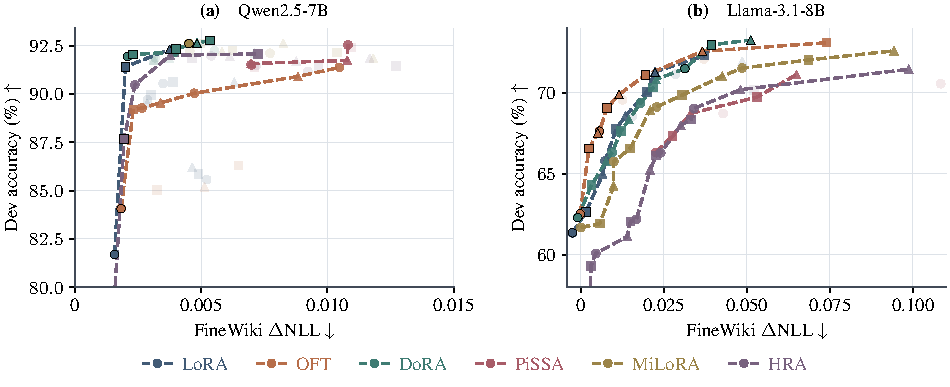
\includegraphics[width=\linewidth]{figures/peft_pareto_full.pdf}
\caption{Six-method mathematics trade-offs, focused on the frontier regions. Each point is a complete capacity/LR configuration, with shapes denoting increasing capacity. Dashed lines and solid points mark within-method frontiers, and black borders mark the pooled frontier. Dominated points are faint. Frontiers use all 89 Qwen and 90 Llama configurations before axis clipping. The later HRA extension and diverged PiSSA configuration are excluded.}
\label{fig:pareto-full}
\end{figure}
\paragraph{Performance and retention across settings.}
Qwen's small test-accuracy differences coexist with different retention costs. Its high-LR, small-rank LoRA selection is an outlier with greater forgetting than the other methods. LoRA's larger-rank selections have less forgetting. HRA's Qwen scores are competitive, and its original-grid Llama scores improve with capacity alongside increasing retention cost. These results support the main finding that competitive task scores can accompany different forgetting costs, with outcomes depending on the selected LR and capacity. Appendix~\ref{app:retention-patterns} summarizes the trends across tasks.
\subsection{Separate HRA learning-rate extension}\label{app:hra-extension}
All three original Llama HRA winners occur at the largest LR, $10^{-3}$. A follow-up therefore adds $3\times10^{-3}$ and $10^{-2}$ at each capacity and seed. The extension was proposed after the original test report and is reported separately. Of 18 training runs, 15 complete both development and official-test evaluations. All three r64 runs at $10^{-2}$ diverge. Selection over the seven-LR development grid chooses $3\times10^{-3}$ at r16/r32 and retains $10^{-3}$ at r64. The main comparison retains the original five-LR selections.
\begin{table}[!htbp]
\caption{Llama-3.1-8B HRA development-selected outcomes after the separate seven-LR follow-up. The r64 selection is unchanged from the original grid. $n$ is the successful seed count. LR selection uses development scores.}
\label{tab:math-hra-extension}
\begin{center}
\setlength{\tabcolsep}{3pt}
\begin{tabular*}{\linewidth}{@{\extracolsep{\fill}}lccccc@{}}\toprule
Adapter & LR & $n$ & Dev (\%) $\uparrow$ & Test (\%) $\uparrow$ & $\Delta$NLL $\downarrow$ \\\midrule
\textcolor{HRAColor}{HRA} r16 & $3\times10^{-3}$ & 3 & $\result{math_extension_llama_hra_16_0p003_dev_mean}_{\pm\result{math_extension_llama_hra_16_0p003_dev_sd}}$ & $\result{math_extension_llama_hra_16_0p003_test_mean}_{\pm\result{math_extension_llama_hra_16_0p003_test_sd}}$ & $\result{math_extension_llama_hra_16_0p003_forgetting_mean}_{\pm\result{math_extension_llama_hra_16_0p003_forgetting_sd}}$ \\
\textcolor{HRAColor}{HRA} r32 & $3\times10^{-3}$ & 3 & $\result{math_extension_llama_hra_32_0p003_dev_mean}_{\pm\result{math_extension_llama_hra_32_0p003_dev_sd}}$ & $\result{math_extension_llama_hra_32_0p003_test_mean}_{\pm\result{math_extension_llama_hra_32_0p003_test_sd}}$ & $\result{math_extension_llama_hra_32_0p003_forgetting_mean}_{\pm\result{math_extension_llama_hra_32_0p003_forgetting_sd}}$ \\
\textcolor{HRAColor}{HRA} r64 & $1\times10^{-3}$ & 3 & $\result{math_grid_llama_hra_64_0p001_dev_mean}_{\pm\result{math_grid_llama_hra_64_0p001_dev_sd}}$ & $\result{math_grid_llama_hra_64_0p001_test_mean}_{\pm\result{math_grid_llama_hra_64_0p001_test_sd}}$ & $\result{math_grid_llama_hra_64_0p001_forgetting_mean}_{\pm\result{math_grid_llama_hra_64_0p001_forgetting_sd}}$ \\
\bottomrule\end{tabular*}
\end{center}
\end{table}
\FloatBarrier
The development-selected $3\times10^{-3}$ extension raises mean test accuracy at both r16 and r32, while increasing their retention costs. At r64, $3\times10^{-3}$ reduces accuracy and increases NLL, so development selection retains the original LR. HRA therefore illustrates the setting-dependent trade-offs in Section~\ref{sec:comparisons}, with the useful LR range changing across capacities.
\FloatBarrier
